\PassOptionsToPackage{unicode}{hyperref}
\PassOptionsToPackage{hyphens}{url}
%
\documentclass[12pt, a4paper]{article}
\usepackage[a4paper,margin=3cm]{geometry}
\setlength\parindent{0pt}
\setlength\parskip{4pt}
\usepackage{mathptmx}
\usepackage{amsmath,amssymb}
\usepackage[T1]{fontenc}
\usepackage[utf8]{inputenc}
\usepackage{textcomp}
\usepackage{booktabs}
\usepackage{graphicx}
\usepackage{array}
\usepackage[font=small,labelfont=bf]{caption}
\usepackage{xurl}
\usepackage[hidelinks]{hyperref}
\graphicspath{{figures/}}

% Tables and figures are generated by the report_assets step: never edit them by hand.
\newcommand{\gentable}[1]{\input{tables/#1}}

\author{Jacopo Bonifazi, Degree Programme, ID number
\\Francesco Castaldi, Master's Degree in Computer Science, ID number
\\Paolo Fusco, Degree Programme, ID number
\\Shivam Kumar, Degree Programme, ID number
\\Gaetano Muscarello, Degree Programme, ID number}
\date{}
\title{Structural Analysis of Professional Tennis Networks:\\
A Comparative Study Across Eras, Surfaces, and Genders}

\begin{document}
\maketitle

\section{Introduction}
\label{introduction}

% Role A (about 450 words). General field (sport analytics, network science applied to sport),
% specific application (networks of matches between players), prior work: Radicchi (2011), Michieli (2018).

\section{Problem and Motivation}
\label{problem-and-motivation}

% Role A (about 500 words). Research question of the outline, why eras, surfaces and tours,
% contributions of the project. Hypotheses H1-H4 are stated in Measures and Results.

\section{Datasets}
\label{datasets}

We work with two public sources and model every one of them in the same way: a node is a professional player, and an edge connects two players who met in at least one official singles match. Unless stated otherwise the edge is directed from the loser to the winner and its weight is the number of times the winner beat the loser in the period, so the in-strength of a player is the number of matches won and the out-strength the number of matches lost. All the networks are one-mode and no node carries attributes other than the ranking described below. Table~\ref{tab:networks} lists the thirteen networks.

\paragraph{Reference networks (Michieli, 2018).} The author of the reference paper~\cite{michieli2018} published four MATLAB adjacency matrices in a public Google Drive folder, which we downloaded on 16 October 2026 together with its readme. Networks M1 to M3 cover the main draw of ATP tournaments from 1968 to August 2017 and share the same 4,245 players in the same order. M1 is the directed wins network described above; the sum of its weights is 151,734, the number of matches reported in the paper. M2 links every pair of opponents in both directions with the ATP points awarded in their matches; contrary to its readme, the two directions carry the same weight in 97\% of the pairs, so M2 holds no information on who won and we do not analyse it further. M3 is the undirected and unweighted version of M1. M4 extends M3 to March 2018 and adds Davis Cup, Challenger and Futures matches from 1991, reaching 22,405 players. The four matrices are aggregated over five decades and carry no match dates, so they cannot be split by era, surface or tour. We use them as a historical baseline and to check that our pipeline reproduces the published figures (Section~\ref{validity-and-reliability}).

\paragraph{Comparative networks (tennis-data.co.uk).} To build sub-networks we need the date and the surface of every match. The archive used by the reference paper (Jeff Sackmann's GitHub repositories) is no longer public, so we turned to tennis-data.co.uk~\cite{tennisdata}, which the paper also cites. It publishes one spreadsheet per season with date, tournament tier, surface, round, the two players and their ATP or WTA ranking on the day of the match. We downloaded the 26 ATP seasons from 2000 to 2025 and the 19 WTA seasons from 2007 to 2025 (the 2026 season is still in progress), and recorded the URL, size and SHA-256 digest of each of the 45 files. Cleaning was limited to three steps. We dropped matches ended by walkover, since no tennis was played, and kept retirements. We normalised white space in player names, which already follow the ``Surname I.'' format of the reference networks. We merged the Greenset surface into hard courts, of which it is a brand, and left out of the surface networks the 1,685 ATP matches played on carpet, a surface abandoned in 2009. The result is 114,084 played matches (68,972 ATP and 45,112 WTA).

From these matches we built nine directed and weighted networks, with the same edge semantics as M1: four ATP eras (2000-2006, 2007-2012, 2013-2018, 2019-2025), the three ATP surfaces over 2000-2025, and the ATP and WTA tours over the common window 2007-2025. The eras are roughly equal in number of matches (15,661 to 20,265), and 2007-2018 spans the seasons dominated by Federer, Nadal and Djokovic. For every network we also stored the median ranking of each player over his or her matches in the period, which we use to compare network centrality with the official ranking and to define ranking bands (top 10, 11 to 100, others).

\paragraph{Tools.} Data are stored as plain CSV edge lists (\texttt{source}, \texttt{target}, \texttt{weight}). We read the MATLAB files with SciPy and a small decoder for the MATLAB string that holds the player names, which SciPy does not parse, and the spreadsheets with pandas. Every measure is computed in Python with NetworkX~3.6~\cite{networkx}, figures are drawn with Matplotlib, and the null models use our own degree-preserving edge swap, ten to twenty times faster than the NetworkX one on these graphs. A single configuration file lists the networks, the number of null samples and the random seed (20261115), which is passed to every random generator. Scripts rebuild the processed files from the raw ones, run all the measures and produce every table and figure of this report, and automated tests check the parsers and the edge counts.

\begin{table}[t]
\centering
\footnotesize
\gentable{tab_networks.tex}
\caption{The networks of the study. M1 to M4 are the reference networks of Michieli (2018); the other nine are built from tennis-data.co.uk. Edges of directed networks go from the loser to the winner.}
\label{tab:networks}
\end{table}

\section{Validity and Reliability}
\label{validity-and-reliability}

To ensure that our empirical findings reflect genuine tennis dynamics rather than artifacts of data processing, we evaluate the validity of our modeling assumptions, verify consistency across independent data sources, reproduce published baseline figures, and enforce automated reproducibility protocols.

\paragraph{Reproduction of the reference paper.}
Table~\ref{tab:reproduction} compares the topological properties obtained by our pipeline against those reported by Michieli~\cite{michieli2018}. Across networks M1, M3 and M4, our computations reproduce the published values almost exactly: the largest strongly connected component of M1 contains precisely 2,428 players, the average geodesic distances match within 0.01 hops (3.47 against 3.48 in M1, 3.34 in M3, 3.63 against 3.64 in M4), and degree assortativities agree closely ($-0.004$ against $-0.008$ in M3, 0.272 in M4). Furthermore, our PageRank ranking on M1 identifies the exact same top ten players reported in the paper (headed by Connors, Lendl, Federer and McEnroe). The only discrepancy lies in average clustering: Michieli reports 0.07 on M3, whereas standard NetworkX formulas yield 0.311 (and a global transitivity of 0.355). We verified that no standard definition of local or global clustering produces 0.07 on this graph, suggesting an unstated normalization or alternative definition in the original work.

\paragraph{Cross-source consistency.}
Because Jeff Sackmann's original repository is no longer accessible, we cross-validated our primary source (\texttt{tennis-data.co.uk}) against Michieli's historical matrix M1 over their overlapping window (ATP main-draw matches from January 2000 to August 2017). Across 32,297 directed loser-winner pairs in our processed dataset, 31,513 (97.6\%) appear identically in M1. Out of 1,360 distinct ATP players active in that period, 1,350 (99.3\%) match M1 directly; manual inspection revealed that the remaining ten players differ solely by minor surname transliterations. This confirms that our comparative networks are drawn from the same competitive population as the reference literature.

\paragraph{Construct validity.}
The network model isolates elite professional performance by restricting edges to official main-draw singles matches, leaving out qualifying rounds and lower-tier tournaments that would introduce heterogeneous skill pools. Walkovers are discarded because no tennis was contested, whereas retirements are retained because competitive play occurred prior to withdrawal. Aggregation over multi-year eras buffers single-season variance while preserving chronological shifts in tour dominance. Player ability is anchored using each player's median official ATP or WTA ranking across their matches in the period, providing an external ground truth that avoids ranking volatility from short injury layoffs.

\paragraph{Reliability and reproducibility.}
Every raw file downloaded from \texttt{tennis-data.co.uk} and Google Drive is pinned by its SHA-256 digest in \texttt{docs/data.md}. All stochastic algorithms, including degree-preserving null models, season permutations and QAP shuffles, use a fixed random seed (20261115). The entire workflow is executed deterministically through Python modules, validated by 44 automated unit tests, formatted via Ruff, and compiled through continuous integration.

\begin{table}[t]
\centering
\footnotesize
\gentable{tab_reproduction.tex}
\caption{Reproduction of the figures of Michieli (2018). Distances on the large networks are estimated from 1,000 random BFS sources.}
\label{tab:reproduction}
\end{table}

\section{Measures and Results}
\label{measures}

Each measure answers one of the questions of Section~\ref{problem-and-motivation}; we group them by the phenomenon they capture and report the values for the nine comparative networks in Table~\ref{tab:global}. Measures that need an undirected graph (clustering, assortativity, $k$-cores) are computed on the projection in which two players are linked if they met at least once.

\paragraph{Size, cohesion and distances.} Density and mean degree tell how many opponents a player meets, the share of players in the largest strongly connected component (SCC) tells how many players can be reached from each other through chains of victories, and the average distance and the diameter of that component measure how integrated the tour is. All the networks are sparse (density between 0.009 and 0.032) yet compact: inside the SCC two players are on average 2.4 to 3.3 wins apart, and never more than nine. About two thirds of the players belong to the SCC; the others are players who never beat (or never lost to) anyone of the core, typically qualifiers who played a handful of main-draw matches. Reciprocity, the share of linked pairs in which both players won at least once, is close to 0.3 everywhere except on grass (0.09), where the short season leaves few rematches. The surface networks have twice the modularity of the eras (0.38 against 0.11 to 0.15) because they span 26 seasons: Louvain communities~\cite{blondel2008} on a long window mostly separate generations of players who never met.

\paragraph{Degree distribution.} Figure~\ref{fig:degree} shows the complementary cumulative distribution of the number of distinct opponents. The curves are concave on a log-log scale and fall sharply after about one hundred opponents, so none of the networks is scale-free. This is what the format of the sport imposes: a draw of 32 to 128 players and a calendar of about twenty tournaments per year cap the number of matches, and only a long career raises it. The four eras overlap almost perfectly, as do the ATP and WTA tours, while the grass network is cut off much earlier because the grass season lasts about five weeks.

\begin{figure}[t]
\centering
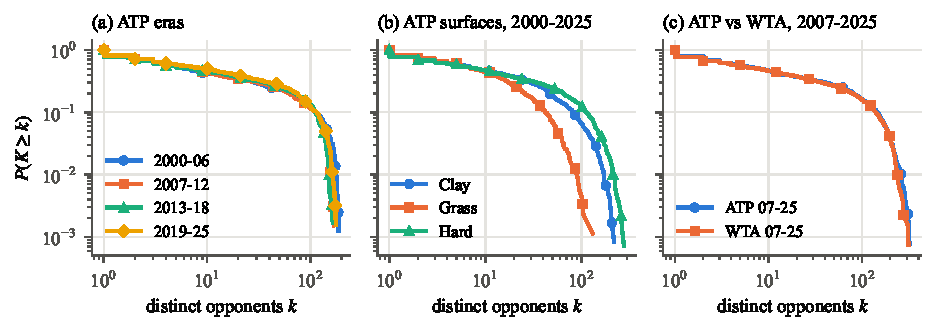
\includegraphics[width=\textwidth]{fig_degree_ccdf.pdf}
\caption{Complementary cumulative distribution of the number of distinct opponents, on log-log axes.}
\label{fig:degree}
\end{figure}

\paragraph{Dominance and prestige.} In-strength counts wins, but a win against a top player should weigh more than one against a qualifier. PageRank~\cite{newman2018} captures exactly this: since edges point from the loser to the winner, a player inherits prestige from the players he or she beat, in proportion to their own prestige, which is the reading proposed for tennis by Radicchi~\cite{radicchi2011}. We summarise the concentration of prestige with the share of total PageRank held by the ten best players, and the inequality of wins with the Gini coefficient of in-strength; Freeman's degree centralization~\cite{freeman1978} measures how far the network is from a star. PageRank agrees closely with the official ranking: the Spearman correlation with the median ranking of each player is between $-0.80$ and $-0.85$ (negative because rank 1 is the best), with grass as the exception at $-0.65$, a sign that results on grass depend on more than overall strength. Table~\ref{tab:top10} lists the top ten of each era, which match the dominant players of the period (Federer in 2000-2006, the Big Three and Murray in 2007-2018, Medvedev, Djokovic, Zverev, Sinner and Alcaraz in 2019-2025). Wins are very unequally distributed (Gini 0.73 to 0.83): most players win few main-draw matches and a small elite wins most of them.

\begin{table}[t]
\centering
\scriptsize
\setlength{\tabcolsep}{3pt}
\gentable{tab_top10.tex}
\caption{The ten players with the highest PageRank in each ATP era and in the WTA network, with their median ranking in the period in brackets.}
\label{tab:top10}
\end{table}

\paragraph{Core and robustness.} The $k$-core decomposition peels away, step by step, the players with fewer than $k$ opponents inside the remaining network; the innermost core is the group of players who all faced many members of the same group. Its depth (54 to 57 in the eras, 19 on grass) shows that every era has a dense inner circle of regular tour players. To see how much the tour depends on that circle we removed players in decreasing order of PageRank and, as a baseline, in random order, tracking the size of the largest connected component (Figure~\ref{fig:robustness}). Random removals erode the network almost linearly, while removing the top 20\% by PageRank halves the largest component and removing 35-40\% disconnects it completely: the periphery of occasional players is held together only through the elite. The 2019-2025 era is the most resilient (60\% of the component left after removing 20\% of the players, against 51-55\% in the earlier eras), which suggests that matches are spread more evenly over a broader group of strong players.

\begin{figure}[t]
\centering
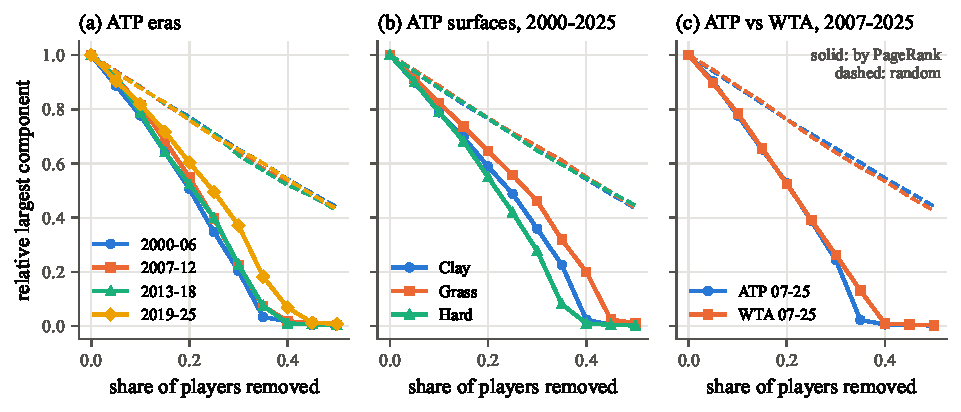
\includegraphics[width=\textwidth]{fig_robustness.pdf}
\caption{Robustness of the networks: relative size of the largest connected component after removing a share of the players in decreasing order of PageRank (solid) or at random (dashed, fixed seed).}
\label{fig:robustness}
\end{figure}

\paragraph{Null models.} Several of these values are partly a consequence of the degree sequence alone. To isolate the effect of the tournament structure we compare them with the configuration model, generated by repeated degree-preserving swaps of two edges~\cite{maslov2002} (ten swaps per edge, 200 samples per network), and report the z-score and the two-sided empirical $p$-value (Table~\ref{tab:null}). The three statistics tell different stories. Degree assortativity is far above the null in every network (the result behind H2 below). Transitivity, the share of closed triangles, is also much higher than expected ($z$ between 23 and 128): when two players have both met a third one, they are likely to have met each other, because strong players keep crossing paths in the late rounds of the same tournaments. Average clustering, which weighs every player equally and is therefore dominated by occasional players with few opponents, is instead slightly below the null in the four eras ($z$ between $-7$ and $-3$) and above it in the surface and WTA networks ($z$ between 6 and 19). Triangles are thus concentrated around the core of the tour rather than spread among peripheral players, which agrees with the robustness results.

\begin{table}[t]
\centering
\footnotesize
\gentable{tab_null.tex}
\caption{Observed values against the configuration model (mean of 200 degree-preserving randomisations of the undirected network) for degree assortativity $r$, average clustering $C$ and transitivity $T$. Every two-sided empirical $p$-value is at most 0.01.}
\label{tab:null}
\end{table}

\paragraph{Hypotheses and tests.} After the exploratory analysis we fixed four hypotheses and one test for each (Table~\ref{tab:tests}). Statistics that depend on the size of the network, such as centralization and PageRank shares, are never compared directly across networks of different size: we either compare seasons, which have similar sizes, or use a permutation test that keeps the size of the groups.

\emph{H1: prestige was more concentrated in the years of the Big Three (2007-2018) than in 2019-2025.} We computed the top-10 PageRank share and the degree centralization of each ATP season and compared the mean of the two groups of seasons with 999 random reassignments of the season labels. The top-10 share is higher in 2007-2018 (0.265 against 0.234), but the difference is not significant ($p=0.06$), and centralization is the same in the two periods ($p=0.76$). Figure~\ref{fig:yearly} shows why: the share peaks in single seasons (2009, 2012, 2015, 2020) rather than over the whole period, and already declines after 2015, when the Big Three still won most of the major titles. With twelve and seven seasons the test has little power, so H1 is not supported but not ruled out either.

\emph{H2: the networks are more disassortative than the configuration model predicts, because in the early rounds strong players meet weak ones.} The observed degree assortativity~\cite{newman2002} is close to zero ($-0.04$ to $0.10$), while the configuration model with the same degrees is clearly disassortative ($-0.19$ to $-0.06$). The difference has the opposite sign of the hypothesis in all eight networks tested (the four eras, the three surfaces and the WTA), with $z$ between 15 and 38. H2 is rejected: given how many matches they play, the strongest players meet each other far more often than chance would allow, which is the effect of seeding and of the later rounds of the draw, where only the best remain.

\emph{H3: the grass network is smaller and more centralized than the clay and hard networks.} Grass is smaller by construction (881 players and 7,693 matches against 1,191 and 22,117 on clay). Its raw degree centralization is even lower, but this comparison is biased by size, so we permuted the surface labels of the matches 199 times, keeping the number of matches per surface, and rebuilt both networks each time. Under this null the expected difference in centralization is $-0.049$ against clay and $-0.067$ against hard, and the observed differences ($-0.030$ and $-0.044$) are significantly higher ($p=0.015$); the top-10 PageRank share is also higher on grass ($p=0.005$ in both comparisons). Once size is taken into account, H3 is supported: grass results are concentrated on fewer players.

\emph{H4: in the WTA the PageRank is less concentrated on the top players than in the ATP.} Comparing the two tours season by season over 2007-2025 with a paired sign-flip test (9,990 random sign assignments), the WTA top-10 share is lower by 0.021 on average ($p=0.016$), while degree centralization does not differ significantly ($p=0.17$). H4 is supported for prestige: the women's tour had fewer dominant players, especially after 2013 (mean share 0.221 against 0.246 in the ATP), whereas in 2007-2012 the two tours were close (0.261 and 0.271).

\begin{table}[t]
\centering
\scriptsize
\setlength{\tabcolsep}{3pt}
\gentable{tab_tests.tex}
\caption{Tests of the hypotheses. A and B are the two groups compared, $E_0$[A$-$B] is the difference expected under the null hypothesis (non-zero when the permuted groups differ in size), $p$ is two-sided. Centralization in H1, H3 and H4 is computed on the undirected network of each season or surface.}
\label{tab:tests}
\end{table}

\begin{figure}[t]
\centering
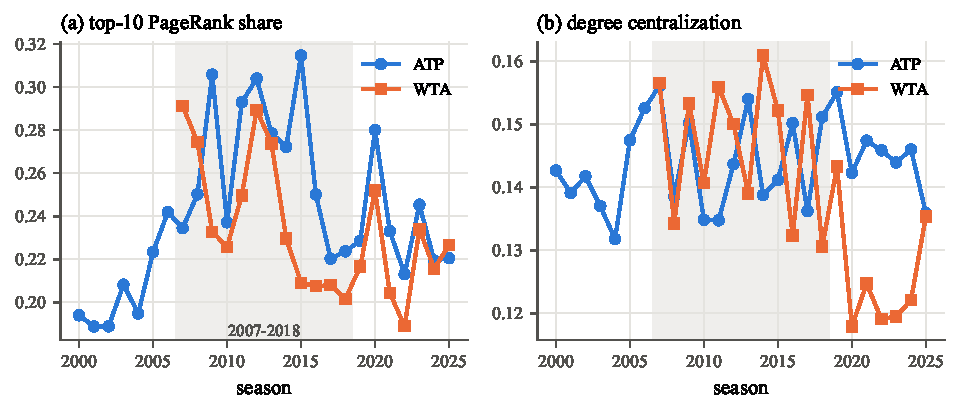
\includegraphics[width=\textwidth]{fig_yearly.pdf}
\caption{Top-10 PageRank share and degree centralization of each season. The shaded area marks the 2007-2018 seasons used in H1.}
\label{fig:yearly}
\end{figure}

\begin{table}[p]
\centering
\scriptsize
\setlength{\tabcolsep}{2.5pt}
\gentable{tab_global.tex}
\caption{Global measures of the nine comparative networks. SCC is the largest strongly connected component; $C$, $T$, $r$ and the $k$-core are computed on the undirected projection; the Spearman coefficient compares PageRank with the median ranking of each player.}
\label{tab:global}
\end{table}

\section{Conclusion}
\label{conclusion}

% Role C (about 450 words). Qualitative reading of the results of the previous section.

\section{Critique}
\label{critique}

% Role C (about 500 words). Limits: main draw only, aggregation by period, size-dependent
% statistics, few seasons for H1, no nationality attribute.

\begin{thebibliography}{9}\small
\bibitem{michieli2018} U.~Michieli. Complex network analysis of men single ATP tennis matches. arXiv:1804.08138, 2018.
\bibitem{tennisdata} tennis-data.co.uk. Historical tennis results and betting odds data. \url{http://www.tennis-data.co.uk/}, accessed 16 October 2026.
\bibitem{radicchi2011} F.~Radicchi. Who is the best player ever? A complex network analysis of the history of professional tennis. \emph{PLoS ONE}, 6(2):e17249, 2011.
\bibitem{newman2018} M.~Newman. \emph{Networks}. Oxford University Press, 2nd edition, 2018.
\bibitem{networkx} A.~Hagberg, D.~Schult, P.~Swart. Exploring network structure, dynamics, and function using NetworkX. In \emph{Proc.\ 7th Python in Science Conference}, 11-15, 2008.
\bibitem{newman2002} M.~Newman. Assortative mixing in networks. \emph{Physical Review Letters}, 89(20):208701, 2002.
\bibitem{maslov2002} S.~Maslov, K.~Sneppen. Specificity and stability in topology of protein networks. \emph{Science}, 296(5569):910-913, 2002.
\bibitem{blondel2008} V.~Blondel, J.-L.~Guillaume, R.~Lambiotte, E.~Lefebvre. Fast unfolding of communities in large networks. \emph{J.\ Stat.\ Mech.}, P10008, 2008.
\bibitem{freeman1978} L.~Freeman. Centrality in social networks: conceptual clarification. \emph{Social Networks}, 1(3):215-239, 1978.
\end{thebibliography}

\end{document}
